\documentclass[letter, 12pt]{article}

\usepackage{amsmath,amsthm,amssymb}
\usepackage{fancyhdr}
\usepackage{geometry}
\usepackage{enumerate}
\usepackage{enumitem}
\usepackage{listings}
\usepackage{algorithm}
\usepackage{hyperref}
\usepackage{algorithmic}
\usepackage{eqparbox}
\usepackage{float}
\usepackage{bm}
\usepackage{bbm}
\usepackage{mathtools}

\author{Shengjie Li}
\title{Homework 3}

\pagestyle{fancy}
\fancyhf{} 
\lhead{Shengjie Li \\ RUID: 188008047}
\cfoot{\thepage} 
\renewcommand{\headrulewidth}{1pt}
\renewcommand{\headwidth}{\textwidth}
\renewcommand\algorithmiccomment[1]{%
	\hfill\#\ \eqparbox{COMMENT}{#1}%
}
\newlist{subquestion}{enumerate}{1}
\setlist[subquestion, 1]{label = \alph*)}

\setlength\parindent{0pt}

% margin adjustment
\addtolength{\textwidth}{1in}
\addtolength{\oddsidemargin}{-0.5in}
\addtolength{\evensidemargin}{-0.5in}
\addtolength{\topmargin}{-.5in}
\addtolength{\textheight}{1.0in}
\setlength\parindent{0cm}

\begin{document}
	\centerline{Homework 3}
	\begin{enumerate}[wide = 0pt, label = \textbf{Problem \arabic*:}]
		\item {\ } 
		\begin{subquestion}
			\item {\textbf{Solution:} }
			\par{The histogram of the 1000 generated random variables is shown in Fig \ref{fig:histo}.}
			\begin{figure}[H]
				\centering
				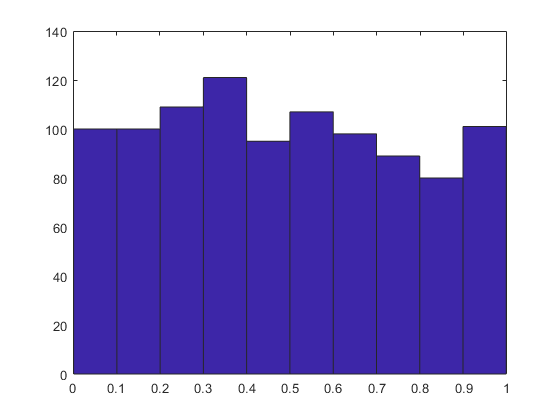
\includegraphics[width=0.7\textwidth]{figs/histogram.png}
				\caption{Histogram of 1000 random variables}
				\label{fig:histo}
			\end{figure}
			\par{According to the Law of Large Numbers, $ \mathbb{E}[K_h(X-x)] \approx \frac{K_h(X - x_1) + K_h(X - x_2) + \dots + K_h(X - x_n)}{n} \approx f(x) $.}
			\par{When we approximate the pdf using the Gaussian kernel, \[ K_h(X) = \frac{e^{-\frac{1}{2h}x^2}}{\sqrt{2 \pi h}}. \] }
			\par{The results are shown in Fig \ref{fig:pdf-gaussian}.}
			\par{We can see from Fig \ref{fig:pdf-gaussian} that when the $ h $ is large, the model underfit the pdf, which is not close enough. As the $ h $ is decreasing, the support of the random variable becomes closer to $ [0, 1] $, and the approximation of pdf becomes more zigzag around 1, starts to overfit.}
			\begin{figure}[H]
				\centering
				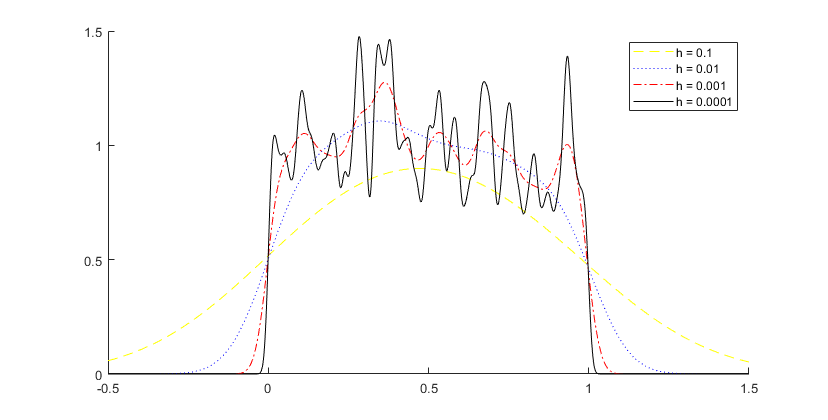
\includegraphics[width=\textwidth]{figs/pdf-gaussian.png}
				\caption{Approximation using Gaussian kernel under different $ h $s.}
				\label{fig:pdf-gaussian}
			\end{figure}
		
			\item {\textbf{Solution:} }
			\par{When we approximate the pdf using the Laplacian kernel, \[ K_h(X) = \frac{e^{-\frac{1}{2h}x^2}}{\sqrt{2 \pi h}}. \] }
			\par{The results are shown in Fig \ref{fig:pdf-laplacian}.}
			\begin{figure}[H]
				\centering
				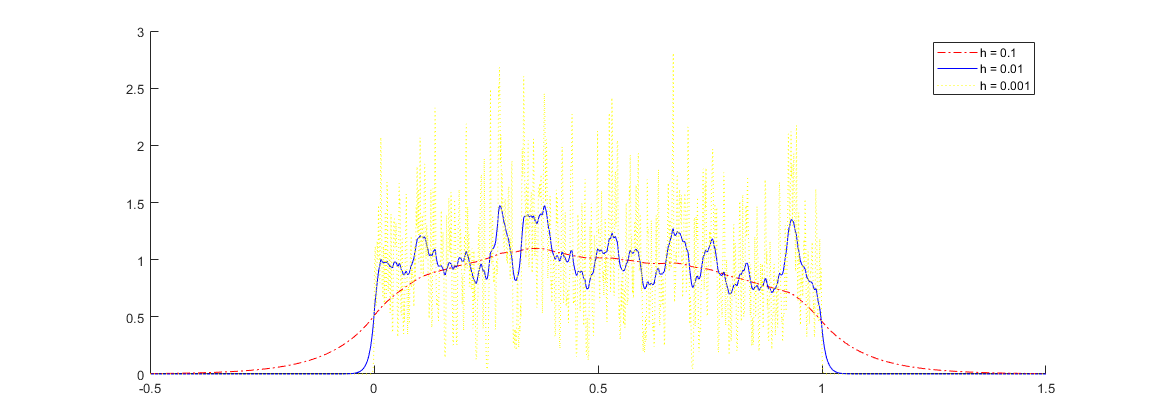
\includegraphics[width=\textwidth]{figs/pdf-laplacian.png}
				\caption{Approximation using Laplacian kernel under different $ h $s.}
				\label{fig:pdf-laplacian}
			\end{figure}
		\end{subquestion}
		
	\end{enumerate}
\end{document}
